\section{External Interface Requirements}
	\subsection{User Interfaces}
		Tickets tonight will follow iOS human interface guideline. Tickets Tonight has two major views, Feed 
		and Explore. The views are contained in a tab bar controller object and the user is given tabs at the 
		bottom of the screen to change into the views. In the Feed view, the user can view events of the artists 
		in their favorites. Each event is displayed as a cell with the image of the event on the left followed by the 
		title and performer text in the middle of the cell. The cells are in iOS table layout. If the user clicks on 
		the cell, then the event information view is displayed in an event view page which displays the image of 
		the event at the top followed by the date of the event, follow toggle for the event (places the event under 
		the following tab in Feed view), the ticket price range, and the location of the event. If the data provides 
		the ticket url, then by clicking on the ticket price cell, the app will start an in-app embedded browser 
		that allows the user to buy the ticket on Ticketmaster’s website. The location of the event is followed by 
		a cell of Apple Maps that pins the event on the map. In the artist view page the user can favorite or 
		unfavorite the artist. The artist page displays the artist name on top followed by his or her picture and 
		event cells of the artist. In the Explore view, the user is presented events of not only his or her favorites 
		but also events of artists recommended by their favorites’ affinity data. The events are displayed in a 
		seemingly flashcard form that the user can swipe away or click on. Each card displays the event image in 
		the top center and the performer image and location at the bottom of the card. The card will also 
		indicate who this artist is similar to. In the more tab, the user can find artists by category and also query 
		all the events that are near his or her current location directly.
		
        \begin{figure}
        \centering
        \begin{minipage}{.5\textwidth}
        	\centering
        	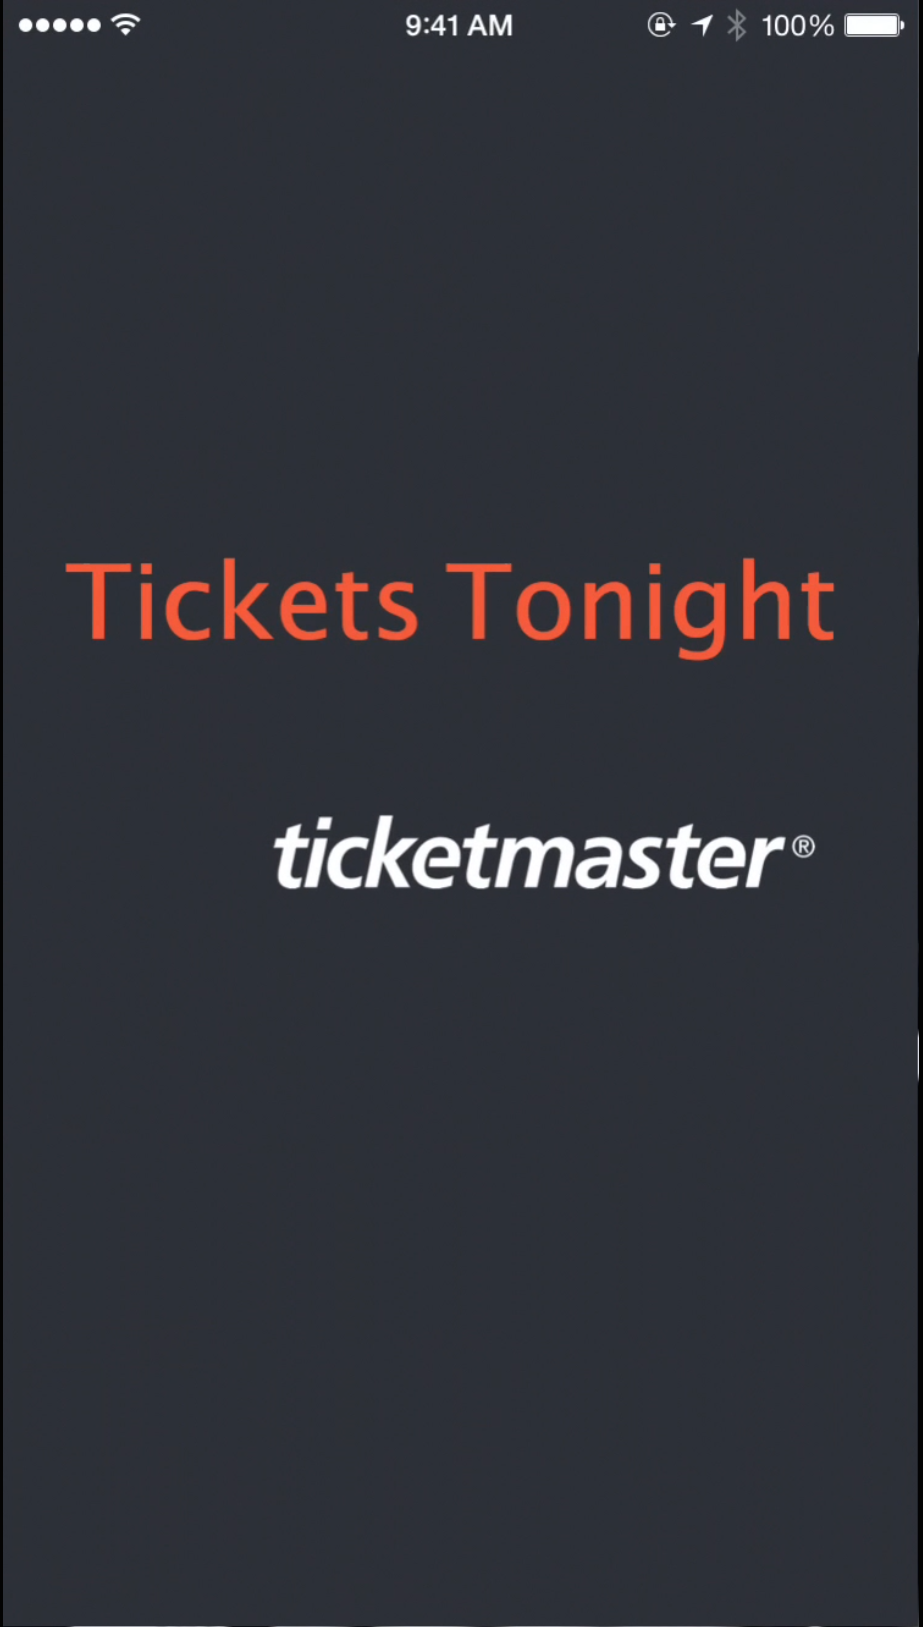
\includegraphics[width=.7\linewidth]{./pics/app1.png}
        	\captionof{figure}{Welcome page}
        \end{minipage}%
        \begin{minipage}{.5\textwidth}
        	\centering
        	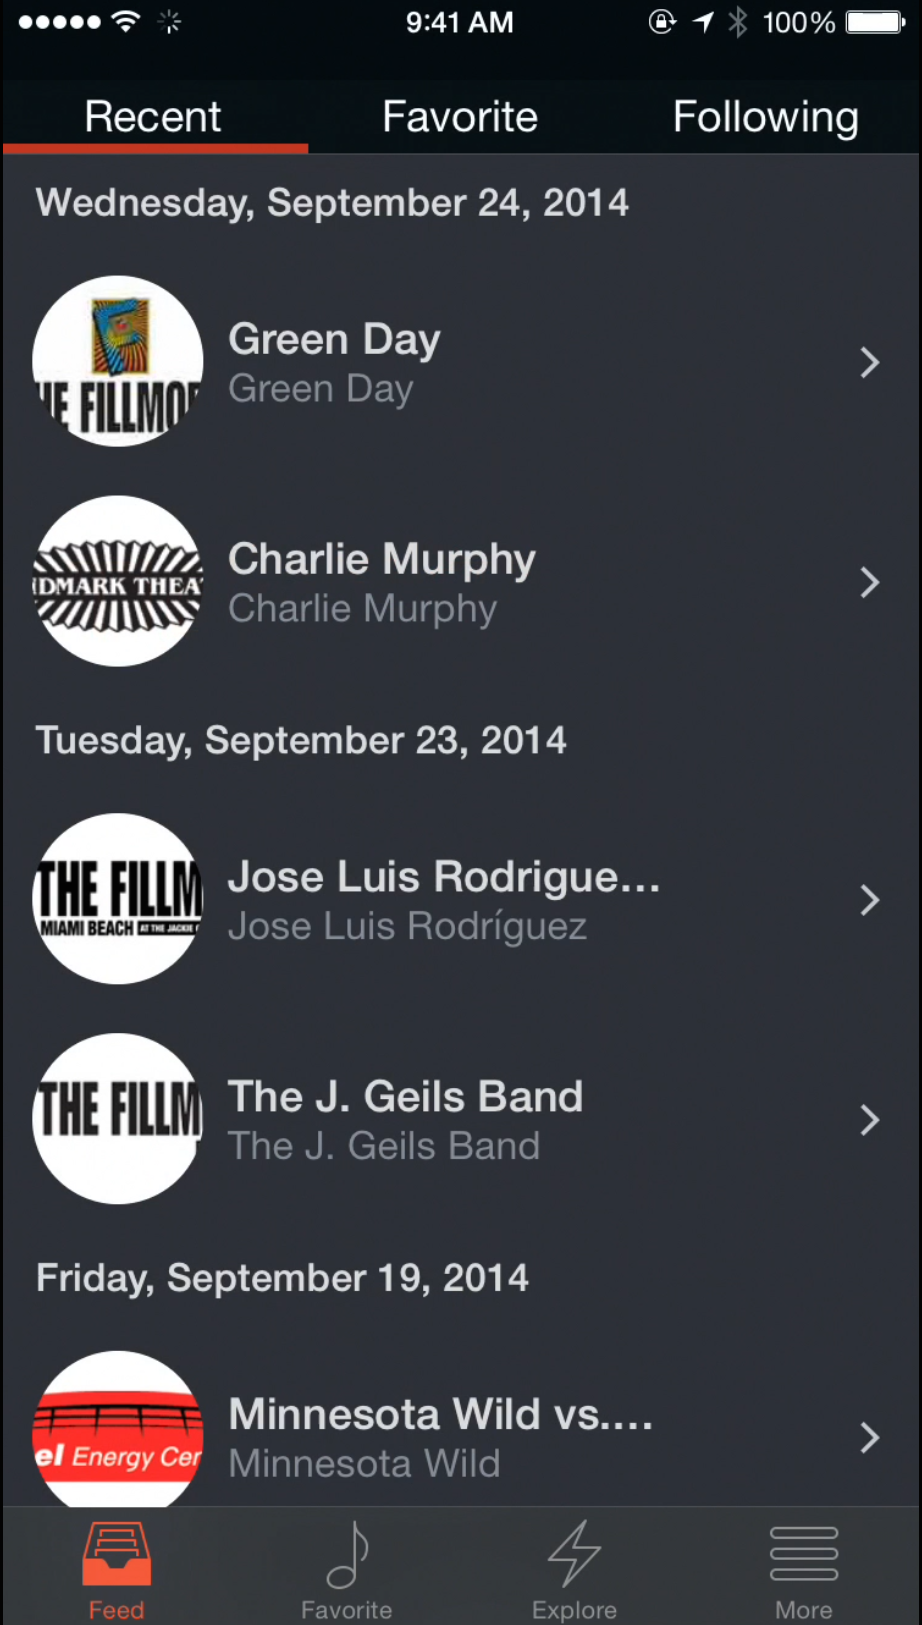
\includegraphics[width=.7\linewidth]{./pics/app2.png}
        	\captionof{figure}{Recent events}
        \end{minipage}
        \end{figure}
        \begin{figure}
        	\centering
        	\begin{minipage}{.5\textwidth}
        		\centering
        		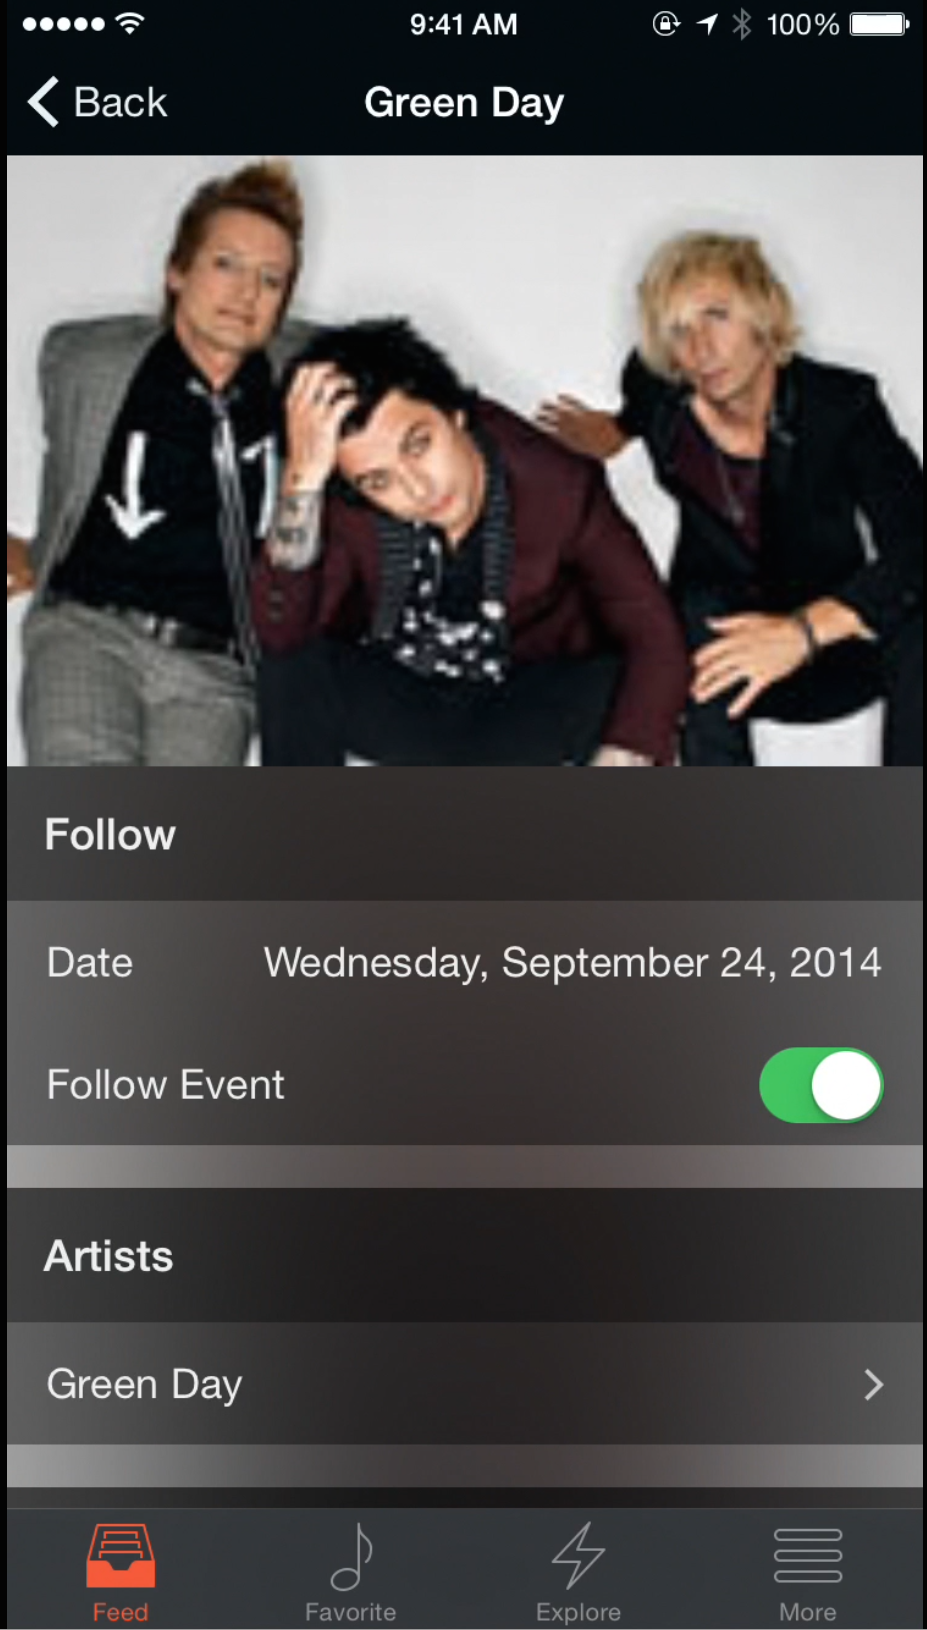
\includegraphics[width=.7\linewidth]{./pics/app3.png}
        		\captionof{figure}{Artist info}
        	\end{minipage}%
        	\begin{minipage}{.5\textwidth}
        		\centering
        		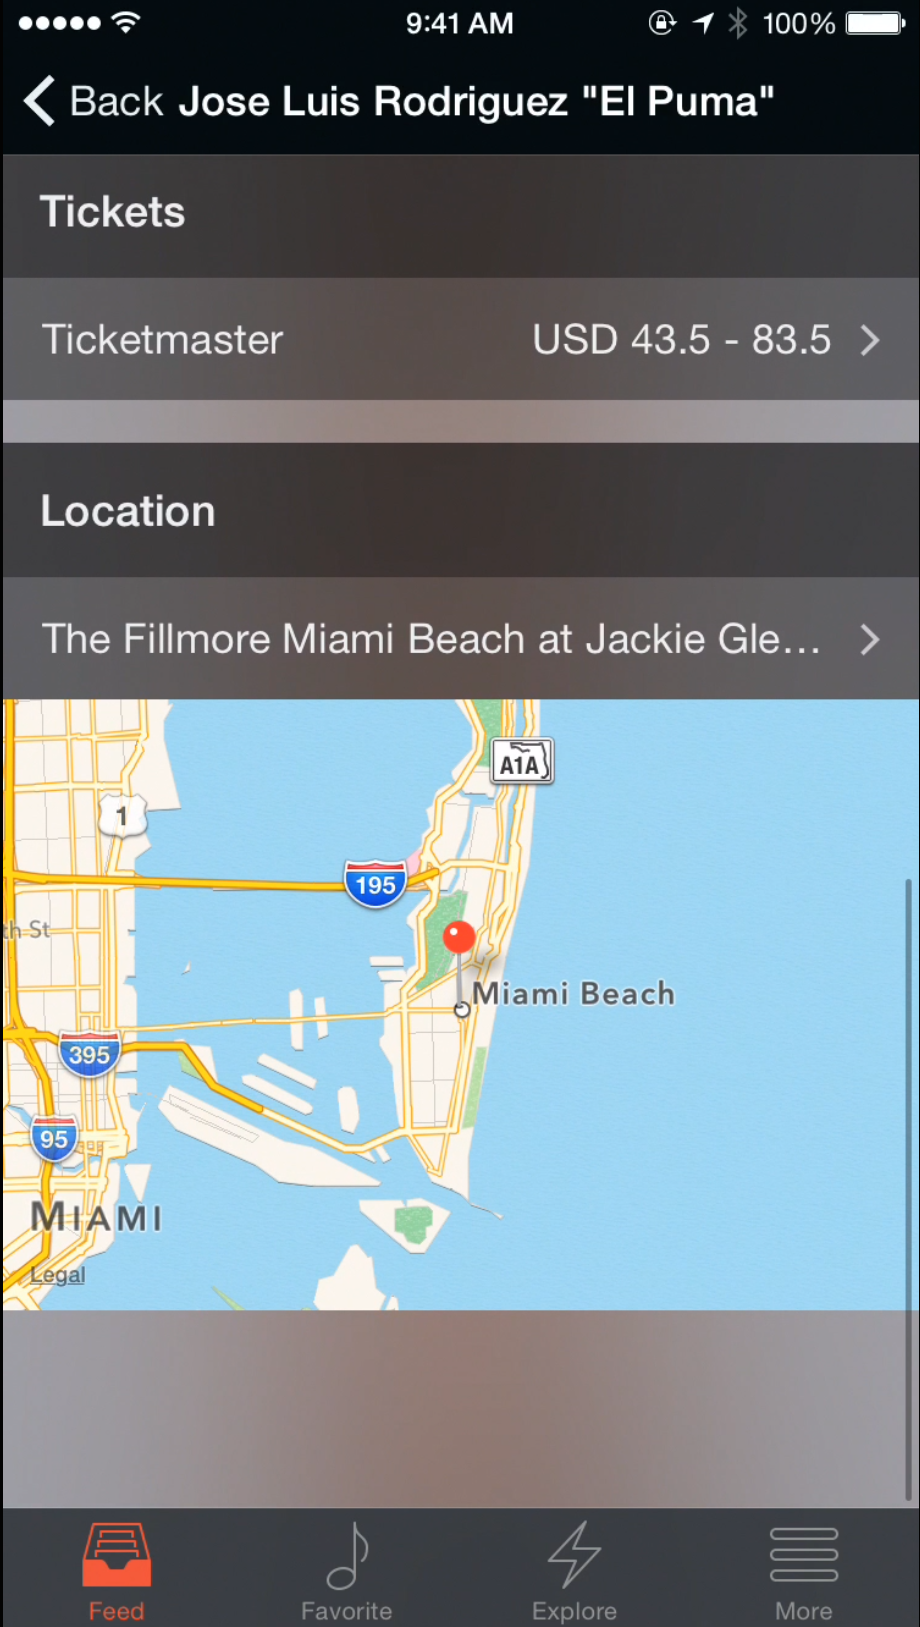
\includegraphics[width=.7\linewidth]{./pics/app4.png}
        		\captionof{figure}{Event location on Apple Maps}
        	\end{minipage}
        \end{figure}		

        \begin{figure}
        	\centering
        	\begin{minipage}{.5\textwidth}
        		\centering
        		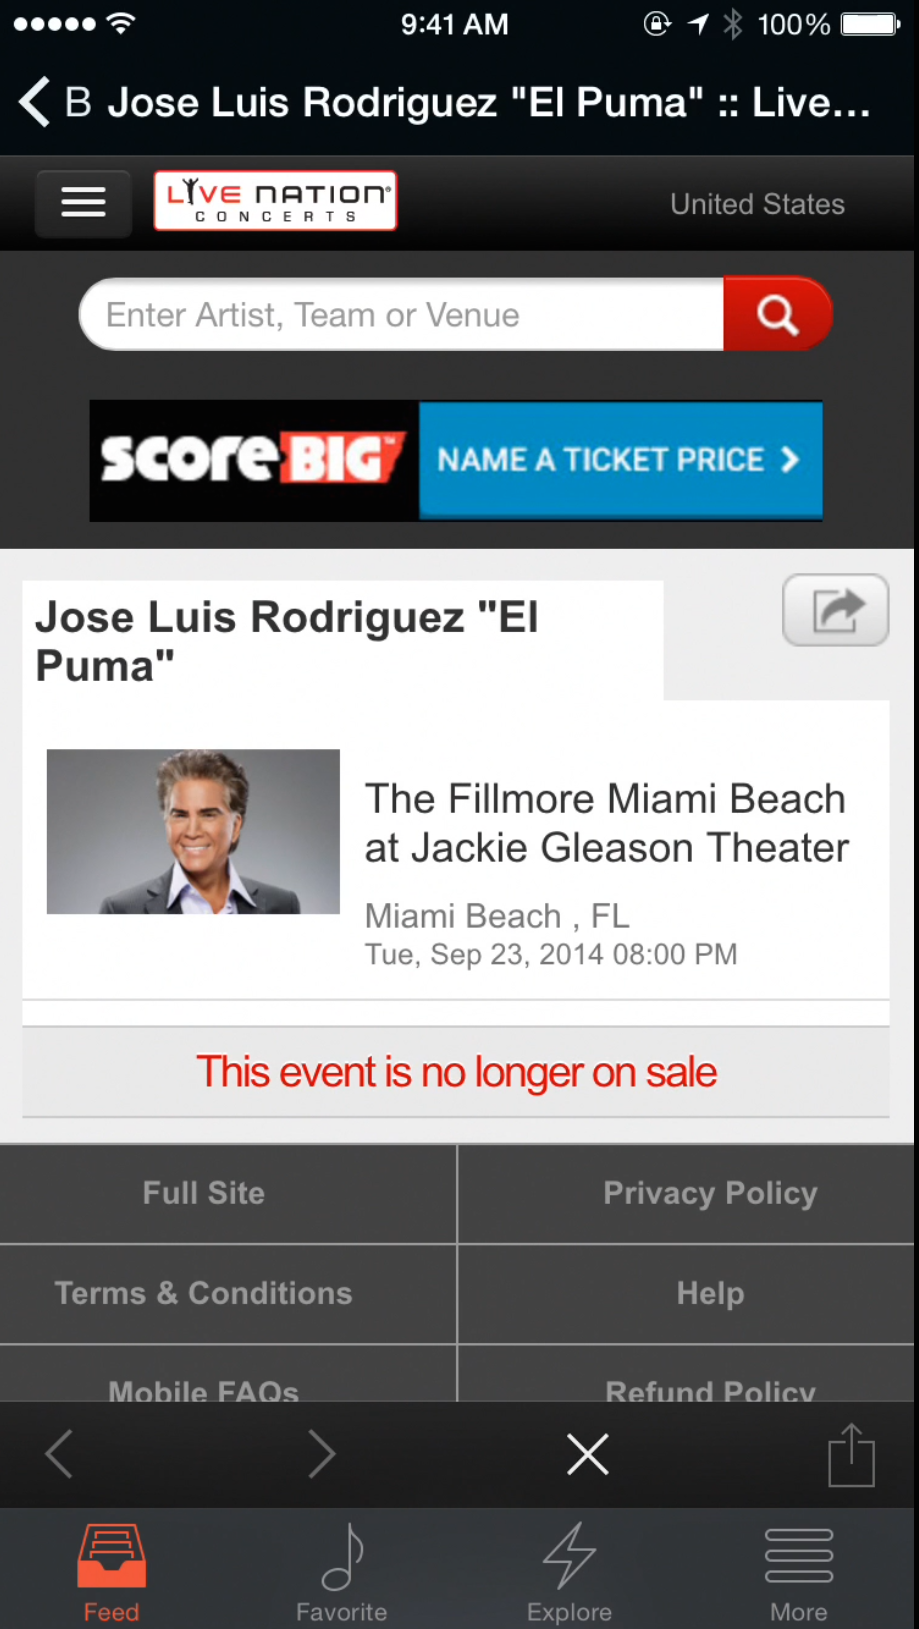
\includegraphics[width=.7\linewidth]{./pics/app5.png}
        		\captionof{figure}{Ticket purchase page}
        	\end{minipage}%
        	\begin{minipage}{.5\textwidth}
        		\centering
        		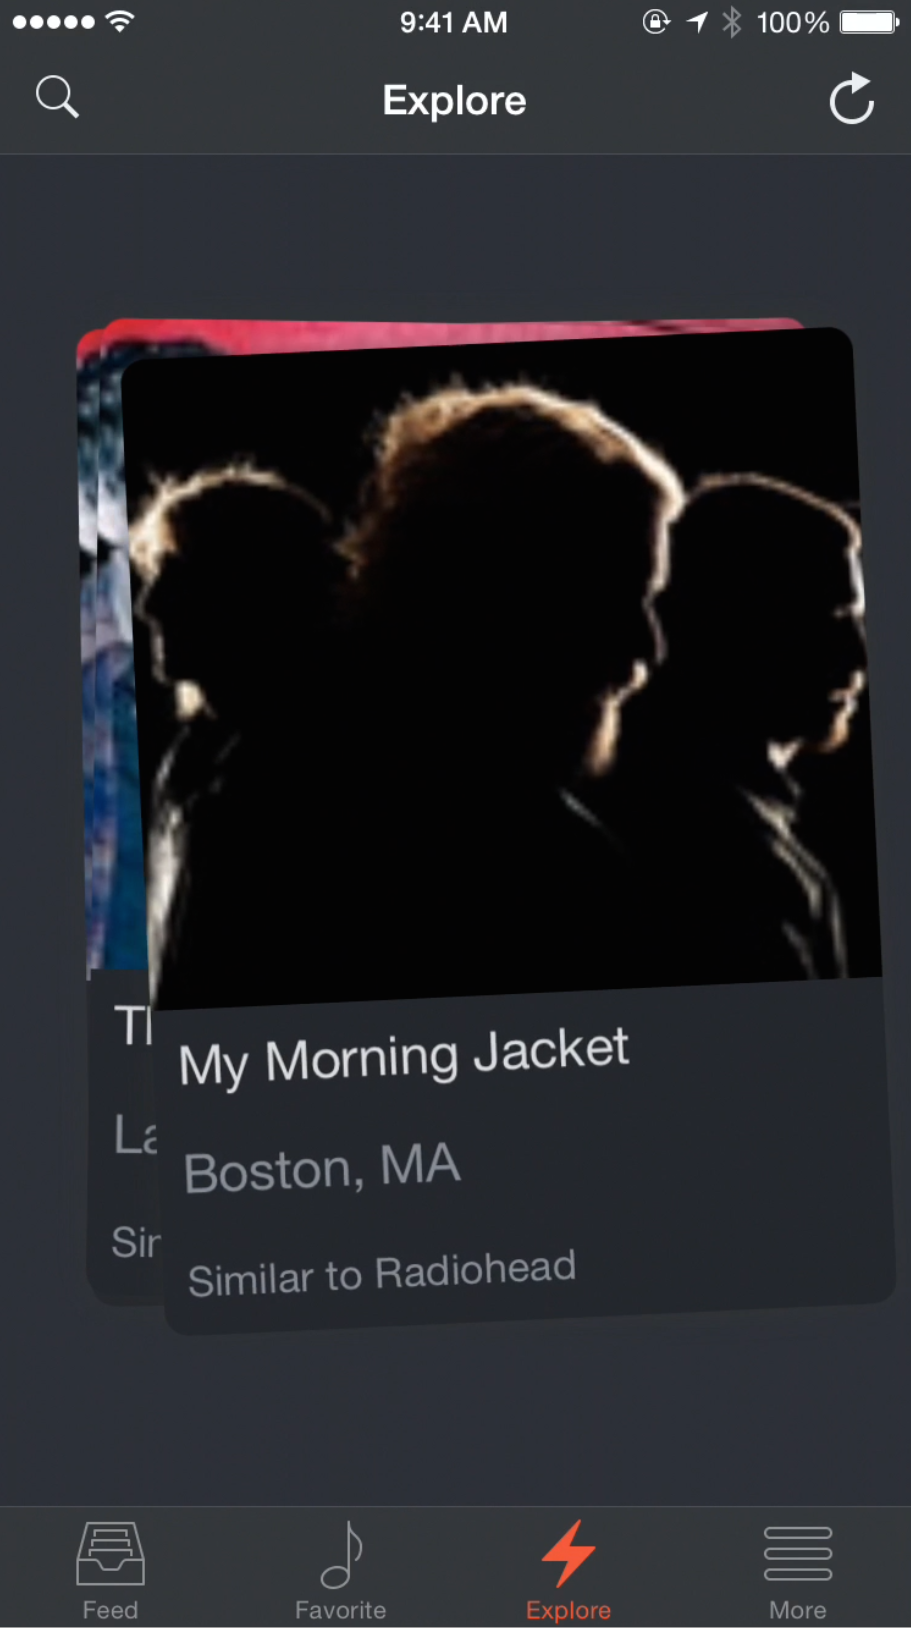
\includegraphics[width=.7\linewidth]{./pics/app6.png}
        		\captionof{figure}{Explore page}
        	\end{minipage}
        \end{figure}		

        \begin{figure}
        	\centering
        	\begin{minipage}{.5\textwidth}
        		\centering
        		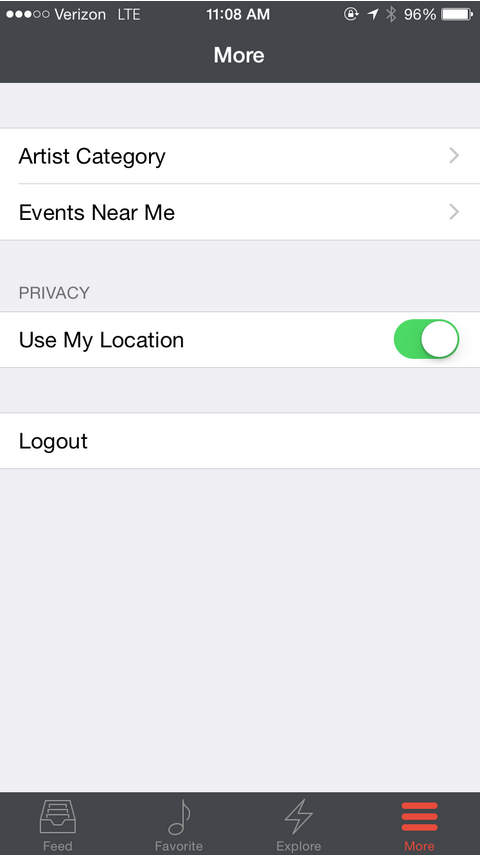
\includegraphics[width=.7\linewidth]{./pics/app7.png}
        		\captionof{figure}{Browse by category}
        	\end{minipage}%
        	\begin{minipage}{.5\textwidth}
        		\centering
        		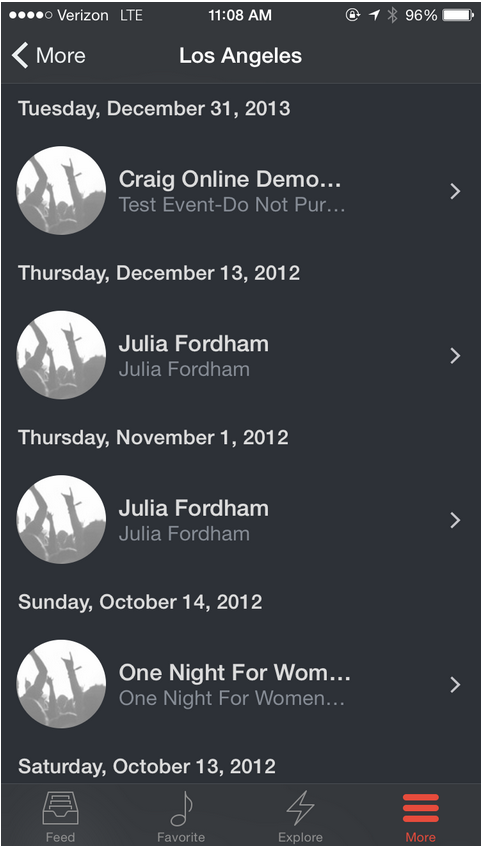
\includegraphics[width=.7\linewidth]{./pics/app8.png}
        		\captionof{figure}{Nearby events}
        	\end{minipage}
        \end{figure}		

	\newpage
	\subsection{Software Interfaces}
	  \subsubsection{Parse Interfaces and Parse iOS SDK}
		Tickets Tonight connects to Parse services in order to access the data provided by Ticketmaster. The Parse iOS SDK connects the app to 
		Parse if the application id and client key is provided. The data from the XML and the affinity text file is parsed by python and stored on 
		Parse as \textit{PFObjects}.  Each \textit{PFObject} contains key-value pairs of JSON-compatible data. This data is schemaless, which means that we 
		don't need to specify ahead of time what keys exist on each \textit{PFObject}. We simply set the key-value pairs we want, and the Parse backend 
		will store it. The \textit{PFObject} has a method to save the data to the Parse backend and the data can be viewed on the Parse app page data 
		browser section. A sample is shown in the following image. 
		\begin{figure}
		\centering
		\begin{minipage}{1.\textwidth}
			\centering
			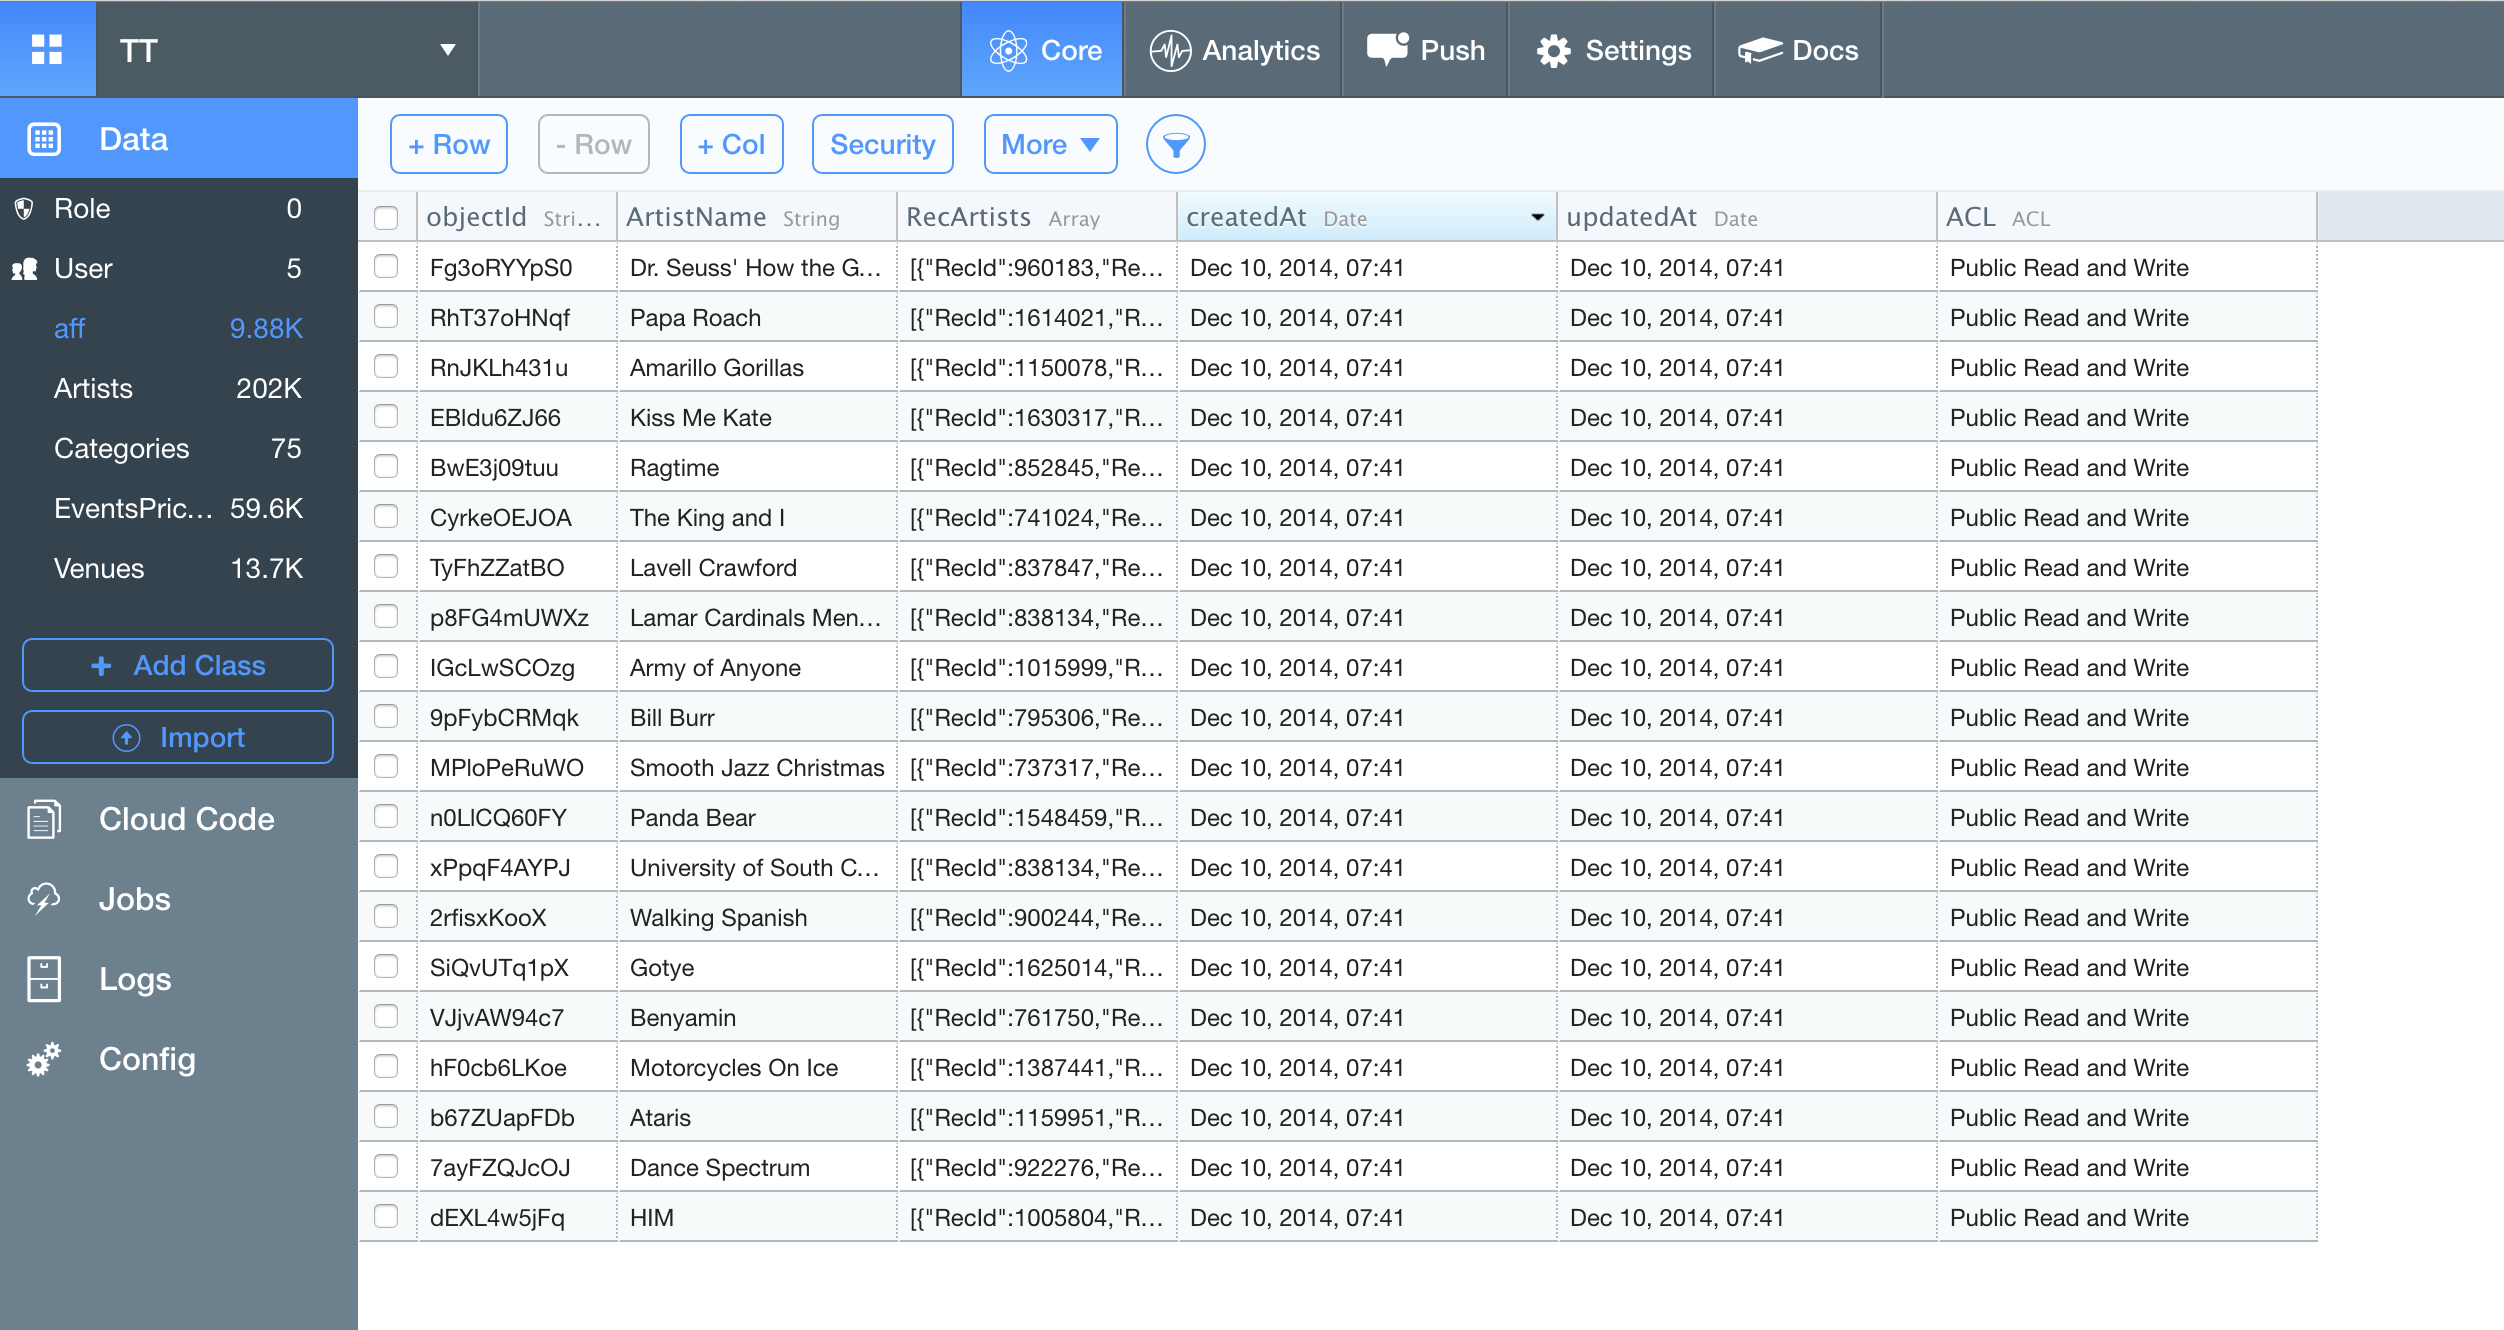
\includegraphics[width=.7\linewidth]{./pics/parse_data_schema.png}
			\captionof{figure}{Data schema on Parse.com}
		\end{minipage}%
	    \end{figure}
	    Tickets Tonight will query the data stored on Parse through a \textit{PFQuery} object that returns the \textit{PFObject} on Parse. 
	    The \textit{PFQuery} can find the \textit{PFObject} if given the object id which will be created as a field when the \textit{PFObject} is instantiated. 
	    Tickets Tonight can save the user’s favorite artists through similar means of querying the \textit{PFObject} and modifying it then saving it. 
	    Saving a \textit{PFObject} to the Parse server can be done offline as well, where we call the \textit{saveEventually} method on the object and the method 
	    will store the update on the device until a network connection is re-established. 
	    
	    The aforementioned interfaces of Parse outlines the overall infrastructure of communication and how Parse is used. More detailed 
	    documentation of each various method and relationships on query and object can be found in References~\ref{reference}
	    The data on Parse are used to generate the cells in the Feed view and the cards in the Explore view. For the Feed view of Tickets Tonight, 
	    we query the user’s favorite artists and then query their events and then order them by date and display in the Feed view. For the Explore 
	    view of Tickets Tonight, we query the user’s favorite artists and then query the affinity data to find recommended artists based on the 
	    user’s favorite artists. Once we have the recommended artists, we query their events and generate the cards for each of their event. When 
	    the user adds an artist to his or her favorite, the data is also saved to Parse. 
	  
	  \subsubsection{iOS Application Interfaces}
	    In the actual application, each view, is handled by the UI Tab Bar controller object. The UI Tab Bar controller object displays a view 
	    corresponding to the tab selected at the bottom of the screen. Each view contained in the tab bar controller object will be linked by the 
	    tab. Under the UI Tab Bar controller object we have a Feed view controller, Favorite view controller, Explore view controller, and settings 
	    view controller. These view controllers are all table view controllers. Table view controllers in iOS displays table cells. We populate the 
	    tables views with Image table view cells which contain an image and text to the right of the image. In the Feed table view controller, we 
	    populate the view with Event cells which contain the image of the event and the title of the event. In Favorite table view controller we 
	    populate the view with artist cells which contain the image of the artist and the name of the artist. The event cells and artist cells lead to 
	    event views and artist views respectively. In the event views we display the image, artist, ticket url and the location of the event. In the 
	    artist views we display the image of the artist and events the artist has. In order to populate the cells with actual data, we query the data 
	    on Parse through the aforementioned Parse interface. By querying Parse with the \textit{PFQuery} object we can obtain the data we need in order 
	    to populate the cells. For detailed description of the object methods, the documentation for view controller objects for iOS is included in 
	    the reference section. In order to display the map in the events page, we convert the address to a geopoint using the \textit{CLGeocoder} object 
	    and using it we could mark the venue on to the map. In order to open the url inside the app, we create a webview to display it. In 
	    addition, when we query the data needed for the explore view, we first obtain the favorite artists objects then flatten them to names in 
	    order to query the affinity data, then acquire recommended artists objects, then flatten those objects into int ID’s, convert those ID’s into 
	    strings, then query the events and finally exclude the events that the user are already following. 
	  	
	  \subsubsection{Python parser}
	    For the data given to us by Ticketmaster, we use Python to parse them into essentially a JSON format to upload to Parse into Parse 
	    objects. For the XML we use the Python library to parse the XML into a tree like objects and create csv objects. For the text file containing 
	    affinity data, which was almost a csv file, we also use the python library to parse it into JSON formatted objects. These objects are then 
	    uploaded to Parse. Parse accepts csv and JSON to populate Parse objects. More detailed description for each of the python library 
	    methods can be found in the reference section. We parse the XML into a csv but the affinity data into JSON because for the affinity data, 
	    an artist can have an array of recommended artists and each artist has a different length of array. CSV requires column number to be the 
	    same for each entry. We could have also put all the recommended artist into one long string in a column for the CSV however, we chose 
	    JSON in order to gain easier access and without having to parse a string. 
	  
	    